\section{Misurazione del traffico: qualche caso di studio}
\subsection{Caratterizzazione del percorso: patchar}
Pathchar \url{ftp://ftp.ee.lbl.gov/pathchar/}
\begin{itemize}
\item Spedisce vari pacchetti (di differenti dimensioni) verso tutti i router, che devono essere analizzati, di un dato percorso.
\item Misura il tempo di risposta pi� breve per ogni hop:
  \begin{itemize}
  \item Ritardo dell'hop.
  \item Larghezza di banda.
  \item Coda
  \end{itemize}
\item Studia il \gls{RTT} respetto alla dimensione del pacchetto, misura la disponibilit� della larghezza di banda.
\item Svantaggi: il test dura troppo. I calcoli sono complessi e necessitano l'invio di un gran numero di pacchetti per dare misurazioni precise.
\end{itemize}

Altri strumenti: pchar, pipechar.

\subsection{Throughput della rete: Iperf}
Iperf \url{http://dast.nlanr.net/Projects/Iperf/}
\begin{itemize}
\item Architettura client/server: qualche binario viene eseguito in due modi differenti.
\item L'applicazione client spedisce al server pacchetti TCP/UDP. Pu� essere specificata la porta, la durata del test, la dimensione della finestra TCP, il volume dei dati del test.
\item Statistiche: larghezza di banda, perdita/ritardo dei pacchetti, jitter.
\item Svantaggi:
  \begin{itemize}
  \item L'applicazione server deve essere installata sull'host di destinazione.
  \item Non lo si pu� installare/usare sui router.
  \end{itemize}
\end{itemize}

\subsection{Di che tipo di report sul traffico abbiamo bisogno?}
\begin{itemize}
\item La top N dei parlatori (chi trasmette molto traffico).
\item La top N delle conversazioni (le coppie di host che si trasmettono molto traffico).
\item La top N delle applicazioni (ad esempio SAP usa il 70\% della larghezza di banda disponibile).
\item Il volume dei dati per entit� di base (link, locazione, regione, classe di utenti).
\item Volume dei dati e velocit� per \gls{AS} (per sapere ad esempio se si ha bisogno di stipulare un nuovo contratto).
\item Marca \gls{QoS} per le applicazioni o per le entit� di base (ad esempio, il \gls{BGP} pu� dire se si sta spedendo il traffico sul percorso migliore?).
\item Rapporti sul traffico che non ci si aspetta di vedere sulla rete (ad esempio perch� l'host X sta spedendo un pacchetto IPX anche se si parla usando solamente IP?).
\end{itemize}

\subsection{Monitoraggio integrato: Cacti}
Cacti \url{http://www.raxnet.net/products/cacti} � uno strumento open source capace di:
\begin{itemize}
\item Collezionare i dati con l'ausilio di metodi SNMP e altri non-SNMP.
\item La configurazione viene fatta via web e la scrittura su un database MySQL.
\item Statistiche salvate in RRD.
\item Estensibilit� attraverso script e XML.
\end{itemize}

\begin{figure}[htbp]
  \centering
  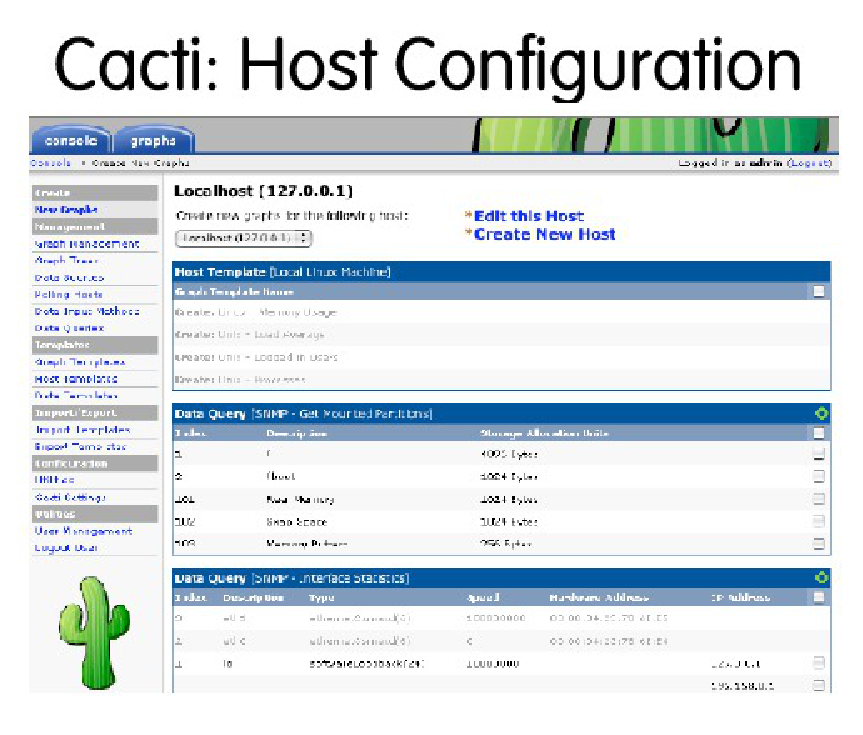
\includegraphics{figure/Cacti_configurazione.eps}
  \caption{Cacti: configurazione}
\end{figure}

\begin{figure}[htbp]
  \centering
  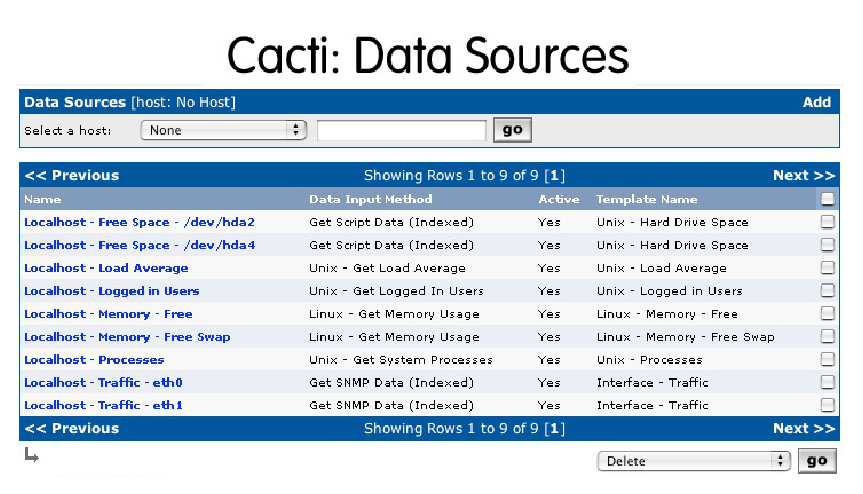
\includegraphics{figure/Cacti_dati.eps}
  \caption{Cacti: dati}
\end{figure}

\begin{figure}[htbp]
  \centering
  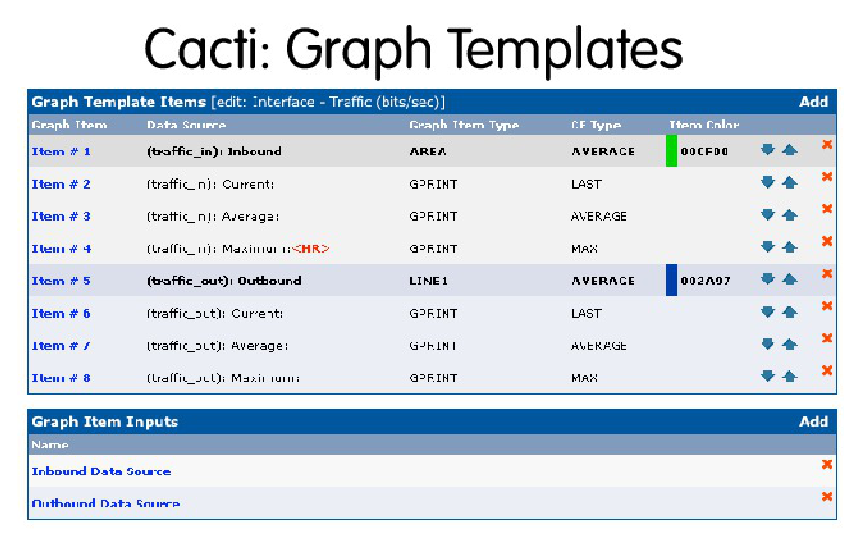
\includegraphics{figure/Cacti_grafico_template.eps}
  \caption{Cacti: grafico dei template}
\end{figure}

\subsection{Caso di studio: gestione della larghezza di banda}
\begin{itemize}
\item I problemi che non sono legati all'acquisto di nuova larghezza di banda ma alla gestione di quella attuale.
  \begin{itemize}
  \item Lezione appresa: pi� larghezza di banda si ha, pi� verr� usata.
  \end{itemize}
  \begin{figure}[htbp]
    \centering
    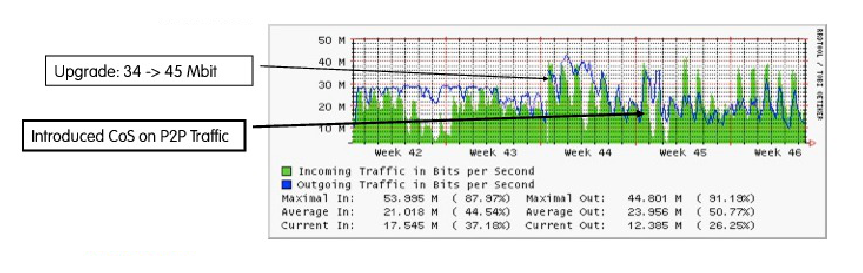
\includegraphics{figure/Gestione_larghezza_di_banda.eps}
    \caption{Gestione della larghezza di banda}
  \end{figure}
\item Soluzione: monitorare e trovare le risposte per le proprie esigenze (non ci sono soluzioni generali).
  \begin{itemize}
  \item Analizzare quanta della larghezza di banda viene utilizzata (ad esempio, perch� viene utilizzato il protocollo X?).
  \item Traffico e matrice del flusso: chi parla con chi e quali dati si scambiano?
  \end{itemize}
\item Lezioni apprese dalla pratica:
  \begin{itemize}
  \item Scarse performance possono essere causate dall'uso dei link di backup perch� quelli primari non sono disponibili (si sta monitorando il failovers - attraverso le trap SNMP - come STP, stato delle porte?).
  \item La rete va bene ma non � al massimo (suboptimal) o � molto dinamica? (SNMP fornisce molti MIB a questo scopo).
  \item Si sta tagliando troppo la banda (shaping\footnote{Lo shaping si effettua introducendo delle classi di servizio (CoS) per impedire che un tipo di traffico monopilizzi tutto.})? Le CoS (Class of Service) sono ottime, ma non se ne dovrebbe abusare (si dovrebbe invece monitorare la quantit� di traffico tagliata dalle proprie politiche)!
  \end{itemize}
\end{itemize}

\subsection{Caso di studio: dov'� un host?}
\begin{itemize}
\item Associazione tra indirizzo IP e nome:
  {\footnotesize
\begin{verbatim}
deri@tar:~$ nslookup 131.114.21.22
   Server: localhost
   Address: 127.0.0.1
   Name: jake.unipi.it
   Address: 131.114.21.22
\end{verbatim}
  }
\item Associazione tra host e proprietario
  \begin{itemize}
  \item namenslookup-type=SOA.
  \item WAIS (Wide Area Information System) \url{http://www.ai.mit.edu/extra/the-net/wais.html}.
  \item  WHOIS [RFC-812].
  \end{itemize}
\end{itemize}

\subsubsection{Esempio di whois}

{\footnotesize
\begin{verbatim}
Domain:         unipi.it
Status:         ACTIVE
Created:        1996-01-29 00:00:00
Last Update:    2008-02-14 00:02:47
Expire Date:    2009-01-29

Registrant
  Name:         Universita' degli Studi di Pisa
  ContactID:    UNIV302-ITNIC
  Address:      Centro SERRA
                Pisa
                56100
                PI
                IT
  Created:      2007-03-01 10:42:01
  Last Update:  2008-01-19 09:46:08

Registrar
  Organization: Consortium GARR
  Name:         GARR-MNT
\end{verbatim}
}

\subsection{Dov'� l'host X nel mondo?}
\begin{itemize}
\item  RFC 1876: un mezzo per Expressing Location Information nel Domain Name System,
\item \url{http://www.caida.org/tools/utilities/netgeo/}
\item \url{http://www.maxmind.com/}
\item \url{http://www.geobytes.com/}
\end{itemize}

\subsection{Caso di studio: impronta digitale degli OS (Operating System - sistema operativo)}
\begin{itemize}
\item Attivo:\\
  Spedire pacchetti di prova per capire il sistema operativo dell'host (\url{http://nmap.org/}).
\item Passivo:\\
  Guardare la stretta di mano a 3 vie (handshake) del TCP e confrontarla con un database di firme conosciute in modo da capire il sistema operativo dell'host (\url{http://ettercap.sf.net/}).
\end{itemize}

\subsubsection{Ettercap}

{\footnotesize
\begin{verbatim}
WWWW:MSS:TTL:WS:S:N:D:T:F:LEN:OS

WWWW: 4 digit hex field indicating the TCP Window Size
MSS : 4 digit hex field indicating the TCP Option Maximum Segment Size
      if omitted in the packet or unknown it is "_MSS"
TTL : 2 digit hex field indicating the IP Time To Live
WS  : 2 digit hex field indicating the TCP Option Window Scale
      if omitted in the packet or unknown it is "WS"
S   : 1 digit field indicating if the TCP Option SACK permitted is true
N   : 1 digit field indicating if the TCP Options contain a NOP
D   : 1 digit field indicating if the IP Don't Fragment flag is set
T   : 1 digit field indicating if the TCP Timestamp is present
F   : 1 digit ascii field indicating the flag of the packet
      S = SYN
      A = SYN + ACK
\end{verbatim}
}

\subsection{Caso di studio: scanner per la sicurezza}
\begin{itemize}
\item Nessus \url{http://www.nessus.org/}.
\item Saint \url{http://www.saintcorporation.com/}.
\end{itemize}

\begin{figure}[htbp]
  \centering
  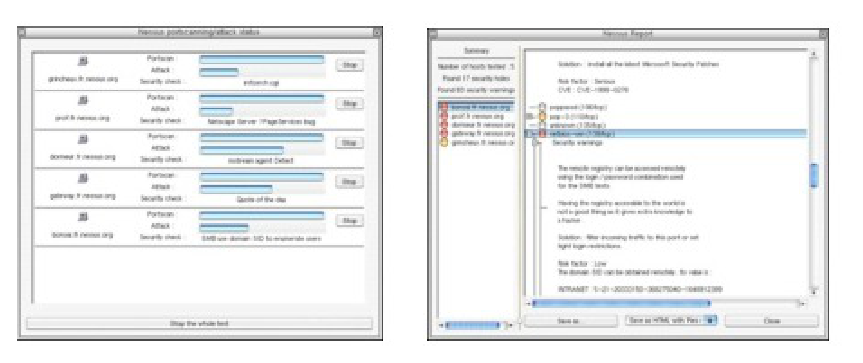
\includegraphics{figure/Scanner_sicurezza.eps}
  \caption{Scanner per la sicurezza}
\end{figure}

\subsection{Caso di studio: sicurezza di rete}
La sicurezza � un processo, non un prodotto (Standard BS 7799, B. Schneier).
\begin{itemize}
\item Si � capaci di determinare le anomalie del traffico?
\item Si � sicuri di sapere cosa monitorare? Molti problemi sono prodotti dal traffico che non ci si aspetta di vedere sulla rete: monitorare ogni cosa, filtrare solo quello che dovrebbe passare, vedere il resto e spiegarsi cos'� successo.
\item Si possiede un meccanismo automatico per recuperare i fallimenti? Si supponga di aver individuato un problema (ad esempio attraverso le trap SNMP) il sistema � capace di reagire in maniera automatica o si deve aspettare il rientro dell'amministratore dalle vacanze?
\end{itemize}

\subsection{Caso di studio: individuazione del traffico \glsentrytext{P2P}}
\begin{itemize}
\item Il \gls{P2P} � difficile da individuare con i metodo classici:
  \begin{itemize}
  \item Non lo si pu� individuare attraverso l'uso di impronte digitali (ad esempio con l'associazione porta-protocollo).
  \end{itemize}
\item Comunque:
  \begin{itemize}
  \item Lo si pu� individuare in termini di modifica di un comportamento standard (ad esempio una workstation non pu� aprire pi� di X connessioni al minuto, e non pu� nemmeno avere pi� di Y connessioni aperte).
  \item Analizzare una parte iniziale del payload per individuare il protocollo.
  \item Alta percentuale di connessione TCP fallite.
  \item Il rapporto pacchetti/byte e sopra la media (le sorgenti \gls{P2P} spediscono molti pacchetti, per lo pi� per parlare con i peer).
  \item Identificare l'esistenza di comunicazione client-a-client (porte $>$ alla 1024) anche se non si hanno canali di comunicazione FTP aperti.
  \end{itemize}
\end{itemize}

\subsection{Caso di studio: individuazione dello SPAM}
\begin{itemize}
\item Reti grandi e aperte (come Universit� o \gls{ISP}) sono il posto migliore dove inviare SPAM (email non richieste).
\item Come identificare la sorgente di SPAM:
  \begin{itemize}
  \item Problema simile all'individuazione del traffico \gls{P2P} ma pi� semplice (solo SMTP, 1 connessione = 1 email).
  \item Selezionare l'insieme dei top N mittenti SMTP.
  \item Rimuovere dall'insieme tutti i server SMTP conosciuti.
  \item Gli studi mostrano che in media gli host non inviano pi� di 8-10 email al minuto.
  \item Un problema veramente semplice da affrontare usando dei protocolli basati sui flusso, come ad esempio NetFlow.
  \end{itemize}
\end{itemize}

\subsection{Caso di studio: individuazione dei virus/trojan}
\begin{itemize}
\item Problema simile all'individuazione dello SPAM ma pi� complesso dato che i protocolli e le porte usate non sono fisse.
\item Gli attacchi non hanno obiettivi mirati: in qualche modo si comportano come scanner di rete.
\item Individuazione:
  \begin{itemize}
  \item Se il problema � conosciuto (ad esempio il traffico sulla porta UDP 135) ci si focalizza su questi traffici.
  \item Buttare un occhio ai messaggi ICMP (ad esempio porta o destinazione non raggiungibile) sono il modo migliore per individuare gli scanner di rete.
  \end{itemize}
\end{itemize}

% LocalWords:  patchar Pathchar router hop dell'hop RTT Trip pchar pipechar TCP
% LocalWords:  Throughput Iperf client UDP jitter sull'host report host SAP AS
% LocalWords:  QoS BGP l'host IPX Cacti source SNMP MySQL RRD template trap STP
% LocalWords:  failovers suboptimal MIB shaping CoS Class of Service type SOA
% LocalWords:  namenslookup WAIS Wide Information System WHOIS RFC whois Domain
% LocalWords:  Expressing Location Name OS Operating dell'host handshake Nessus
% LocalWords:  Ettercap BS Schneier payload peer FTP SPAM SMTP NetFlow trojan
% LocalWords:  ICMP
